%%%%%%%%%%%%%%%%%%%%%%%%%%%%%%%%%%%%%%%%%
% Arsclassica Article
% LaTeX Template
% Version 1.1 (10/6/14)
%
% This template has been downloaded from:
% http://www.LaTeXTemplates.com
%	
% Original author:
% Lorenzo Pantieri (http://www.lorenzopantieri.net) with extensive modifications by:
% Vel (vel@latextemplates.com)
%
% License:
% CC BY-NC-SA 3.0 (http://creativecommons.org/licenses/by-nc-sa/3.0/)
%
%%%%%%%%%%%%%%%%%%%%%%%%%%%%%%%%%%%%%%%%%

%----------------------------------------------------------------------------------------
%	PACKAGES AND OTHER DOCUMENT CONFIGURATIONS
%----------------------------------------------------------------------------------------



\documentclass[
10pt, % Main document font size
a4paper, % Paper type, use 'letterpaper' for US Letter paper
oneside, % One page layout (no page indentation)
%twoside, % Two page layout (page indentation for binding and different headers)
headinclude,footinclude, % Extra spacing for the header and footer
BCOR5mm, % Binding correction
]{scrartcl}



\newcommand*{\Value}{\frac{1}{2}x^2}%
\newcommand*{\inlinecode}{\texttt}%


\usepackage[dvipsnames]{xcolor}
\usepackage{graphicx}
\usepackage{pdfpages}
\usepackage{epsfig} % for postscript graphics files
\usepackage{mathptmx} % assumes new font selection scheme installed
\usepackage{times} % assumes new font selection scheme installed
\usepackage{amsmath} % assumes amsmath package installed
\usepackage{amssymb}  % assumes amsmath %package installed
%\usepackage{subcaption}

\usepackage{mathtools}
\usepackage[portuguese]{babel}
%\usepackage[final]{pdfpages}

\DeclarePairedDelimiter\abs{\lvert}{\rvert}%
\DeclarePairedDelimiter\norm{\lVert}{\rVert}%

\makeatletter
\let\oldabs\abs
\def\abs{\@ifstar{\oldabs}{\oldabs*}}
%
\let\oldnorm\norm
\def\norm{\@ifstar{\oldnorm}{\oldnorm*}}
\makeatother



%%%%%%%%%%%%%%%%%%%%%%%%%%%%%%%%%%%%%%%%%
% Arsclassica Article
% Structure Specification File
%
% This file has been downloaded from:
% http://www.LaTeXTemplates.com
%
% Original author:
% Lorenzo Pantieri (http://www.lorenzopantieri.net) with extensive modifications by:
% Vel (vel@latextemplates.com)
%
% License:
% CC BY-NC-SA 3.0 (http://creativecommons.org/licenses/by-nc-sa/3.0/)
%
%%%%%%%%%%%%%%%%%%%%%%%%%%%%%%%%%%%%%%%%%

%----------------------------------------------------------------------------------------
%	REQUIRED PACKAGES
%----------------------------------------------------------------------------------------

\usepackage[
nochapters, % Turn off chapters since this is an article        
beramono, % Use the Bera Mono font for monospaced text (\texttt)
eulermath,% Use the Euler font for mathematics
pdfspacing, % Makes use of pdftex’ letter spacing capabilities via the microtype package
dottedtoc % Dotted lines leading to the page numbers in the table of contents
]{classicthesis} % The layout is based on the Classic Thesis style

\usepackage{arsclassica} % Modifies the Classic Thesis package

\usepackage[T1]{fontenc} % Use 8-bit encoding that has 256 glyphs

\usepackage[utf8]{inputenc} % Required for including letters with accents

\usepackage{graphicx} % Required for including images
\graphicspath{{Figures/}} % Set the default folder for images

\usepackage{enumitem} % Required for manipulating the whitespace between and within lists

\usepackage{lipsum} % Used for inserting dummy 'Lorem ipsum' text into the template

\usepackage{subfig} % Required for creating figures with multiple parts (subfigures)

\usepackage{amsmath,amssymb,amsthm} % For including math equations, theorems, symbols, etc

\usepackage{varioref} % More descriptive referencing

%----------------------------------------------------------------------------------------
%	THEOREM STYLES
%---------------------------------------------------------------------------------------

\theoremstyle{definition} % Define theorem styles here based on the definition style (used for definitions and examples)
\newtheorem{definition}{Definition}

\theoremstyle{plain} % Define theorem styles here based on the plain style (used for theorems, lemmas, propositions)
\newtheorem{theorem}{Theorem}

\theoremstyle{remark} % Define theorem styles here based on the remark style (used for remarks and notes)

%----------------------------------------------------------------------------------------
%	HYPERLINKS
%---------------------------------------------------------------------------------------

\hypersetup{
%draft, % Uncomment to remove all links (useful for printing in black and white)
colorlinks=true, breaklinks=true, bookmarks=true,bookmarksnumbered,
urlcolor=webbrown, linkcolor=RoyalBlue, citecolor=webgreen, % Link colors
pdftitle={}, % PDF title
pdfauthor={\textcopyright}, % PDF Author
pdfsubject={}, % PDF Subject
pdfkeywords={}, % PDF Keywords
pdfcreator={pdfLaTeX}, % PDF Creator
pdfproducer={LaTeX with hyperref and ClassicThesis} % PDF producer
} % Include the structure.tex file which specified the document structure and layout

\hyphenation{Fortran hy-phen-ation} % Specify custom hyphenation points in words with dashes where you would like hyphenation to occur, or alternatively, don't put any dashes in a word to stop hyphenation altogether



%----------------------------------------------------------------------------------------
%	TITLE AND AUTHOR(S)
%----------------------------------------------------------------------------------------

\title{\normalfont\spacedallcaps{Relatório Final de IC}} % The article title

\author{\spacedlowsmallcaps{Francisco Muniz}} % The article author(s) - author affiliations need to be specified in the AUTHOR AFFILIATIONS block

\date{\today} % An optional date to appear under the author(s)

%----------------------------------------------------------------------------------------

\begin{document}

%----------------------------------------------------------------------------------------
%	HEADERS
%----------------------------------------------------------------------------------------

\renewcommand{\sectionmark}[1]{\markright{\spacedlowsmallcaps{#1}}} % The header for all pages (oneside) or for even pages (twoside)
%\renewcommand{\subsectionmark}[1]{\markright{\thesubsection~#1}} % Uncomment when using the twoside option - this modifies the header on odd pages
\lehead{\mbox{\llap{\small\thepage\kern1em\color{halfgray} \vline}\color{halfgray}\hspace{0.5em}\rightmark\hfil}} % The header style

\pagestyle{scrheadings} % Enable the headers specified in this block

%----------------------------------------------------------------------------------------
%	TABLE OF CONTENTS & LISTS OF FIGURES AND TABLES
%----------------------------------------------------------------------------------------
%\lipsum[1-15]
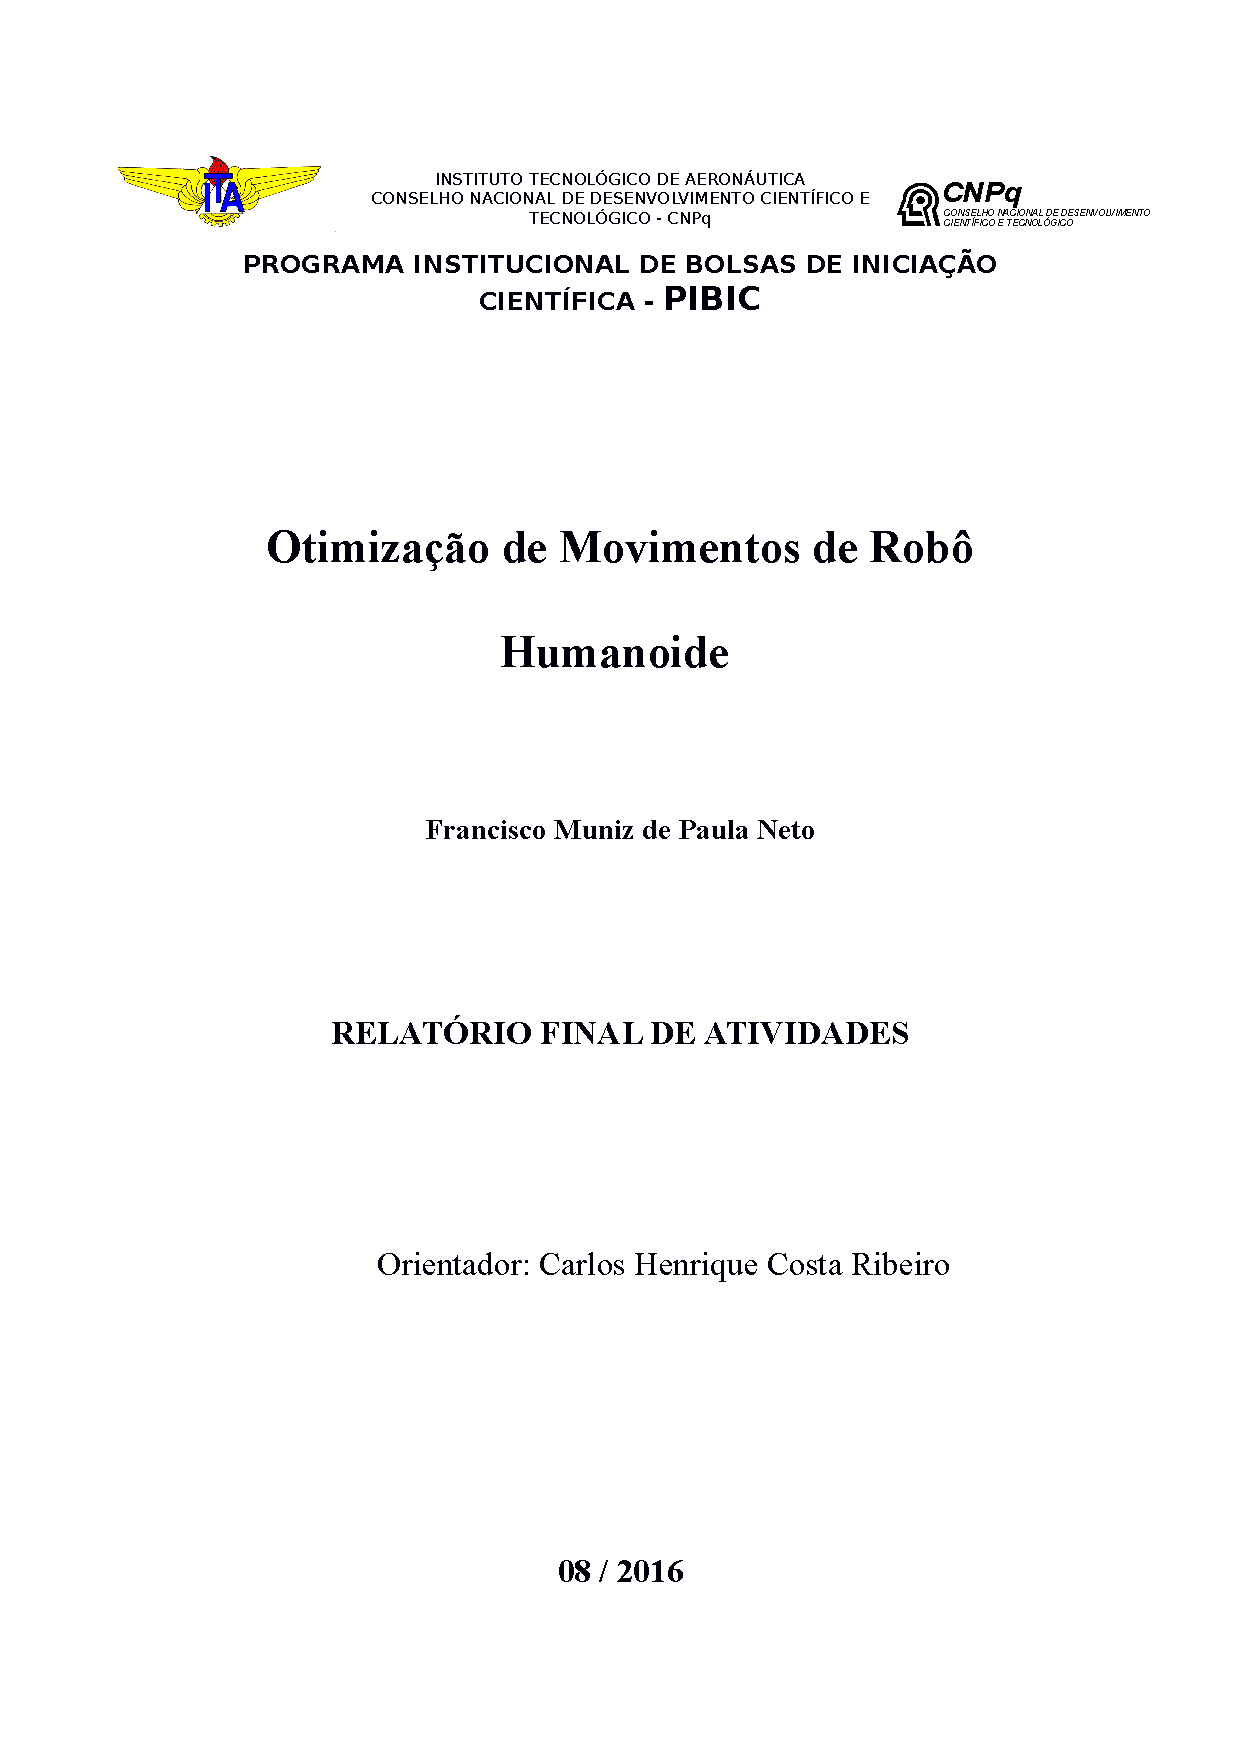
\includepdf[pages={1-},scale=0.75]{test.pdf}

\newpage

\setcounter{tocdepth}{2} % Set the depth of the table of contents to show sections and subsections only

\tableofcontents % Print the table of contents

\listoffigures % Print the list of figures

\listoftables % Print the list of tables

%----------------------------------------------------------------------------------------

\newpage % Start the article content on the second page, remove this if you have a longer abstract that goes onto the second page
 
%----------------------------------------------------------------------------------------
%	RESUMO DO PLANO INICIAL
%----------------------------------------------------------------------------------------

\section{Resumo do Plano Inicial}

O plano inicial era focado em fazer um estudo sobre os movimentos a serem otimizados e, utilizando-se do trabalho anteriormente desenvolvido, para paralelizar os algoritmos e fazer a otimização rodar mais rápido, rodar os algoritmos de otimização sobre tais movimentos e melhorar os resultados do time de Soccer3D do time da ITAndroids.
Deveria-se utilizar uma estratégia para reduzir a quantidade de variáveis a
serem otimizadas, para acelerar a otimização.


%----------------------------------------------------------------------------------------
%	RESUDO DAS ATIVIDADES REALIZADAS
%----------------------------------------------------------------------------------------

\section{Resumo das Atividades Realizadas}

Selecionou-se o uso de movimentos keyframe para otimização, dando maior disponibilidade para o robô 

Foram realizadas várias otimizações, para fazer com que fosse possível do time ter movimentos robustos, que não falhassem numa situação de jogo. 
Não foi possível fazer comparações numéricas sobre o time utilizado pois o time não estava em condições apropriadas para rodar partidas contra outros times, devido a defeitos recentemente solucionados. 

%----------------------------------------------------------------------------------------
%	DESCRIÇÃO DO PROBLEMA
%----------------------------------------------------------------------------------------

\section{Descrição do Problema}

\subsection{Problema de Otimização}

Um problema de otimização matemática consiste em achar o vetor \( \mathrm{\mathbf{x}} \) que minimiza ou maximiza uma certa função objetivo \( f\left( \mathrm{\mathbf{x}} \right) \). Será considerado que estamos interessados apenas em minimizar uma certa função, chamada função de custo, dado que maximizar uma função \( f\left( \mathrm{\mathbf{x}} \right) \) pode ser feito minimizando  \( - f \left( \mathrm{\mathbf{x}} \right) \).





Algoritmos de Otimização Meta Heurística mostram resultados muito bons em resolver problemas de otimização na prática, como pode ser visto em \cite{LNAI14-Depinet} e \cite{rei2010optimizing}. Tais algoritmos normalmente necessitam de pouco conhecimento sobre a função que estão tentando otimizar, sendo necessário computar \( f\left( \mathrm{\mathbf{x}} \right) \) dado \( \mathrm{\mathbf{x}} \). Um problema de tais algoritmos é a falta de garantia de convergência para o mínimo global, e uma convergência para um mínimo local costuma ser vista em tais algoritmos.

\subsection{Representação dos Movimentos Keyframe}


\subsubsection{Keyframe}
Um keyframe $\mathrm{\mathbf{k}} = \left( j_{1}, j_{2}, \dots, j_{n} \right) \in K \subseteq \mathbb{R}^{n} $ é um conjunto ordenado de posições angulares de junta, onde \( K \) e \( n \) são, respectivamente, o espaço de juntas e o número de graus de liberdade do robô.

\subsubsection{Passo de Keyframe}

Um passo de keyfarme é um par $\mathrm{\mathbf{s}} = \left( \mathrm{\mathbf{k}}, t \right) \in S = K \times \mathbb{R} $, onde \( t \) representa o tempo em que o keyframe deve ser alcançado em relação ao início do movimento.


\subsubsection{Movemento Keyframe}
Um movimento keyframe, ou simplesmente um movimento, é definido como $\mathrm{\mathbf{m}} = \left( \mathrm{\mathbf{s}}_1, \mathrm{\mathbf{s}}_2, \dots, \mathrm{\mathbf{s}}_{\gamma}, r \right) \in M=S^{\gamma}\times\mathbb{R}$, onde $\gamma$ é o número de passos associados ao movimento  e \( r \) representa a taxa de velocidade do movimento. Além disso, sempre se considera um movimento começando no tempo 0, i.e. \( t_1 = 0 \). Por isso, cada tempo \( t_i \) representa o tempo em relação ao início do movimento.

Baseia-se a representação de tais keyframes pelas dadas em \cite{rei2010optimizing} e \cite{LNAI14-Depinet}.

\subsection{Movimentos Keyframe}

Movimentos keyframe rodam em um sistema de controle aberto, onde as posições das juntas são obtidas pela interpolação de passos de keyframe, baseando-se no tempo atual da simulação. As juntas do NAO simulado do simulador Simspark são juntas de velocidade, portanto são usados simples controladores proporcionais para cada junta, para acompanhar as posições de juntas, que são necessárias para rodar o movimento keyframe.

Para obter posições de juntas que variam suavemente, interpolam-se os passos de keyframe utilizando splines cubicas como vistas em \cite{Bartels:1987:ISU:35072}, que garantem derivadas de primeira e segunda ordem contínuas. Fig.  \ref{fig:keyframeData} mostra as posições de juntas obtidas a partir da interpolação por splines cubicas; passos de keyframe são mostrados em preto.

Note que achar a interpolação por spline cúbica requer resolver um problema de sistema de equações lineares tridiagonais que pode ser resolvido em \( O(n) \). Entretanto, dado que passos de keyframe são fixos para cada movineot, a interpolação pode ser computada offline. Com isso, achar a interpolação atual pode ser achada em \( O(1) \) dado que os passos de keyframe são utilizados sequencialmente duranto o movimento: Mantém-se um iterador para a interpolação atual e atualiza-se esse iterador quando o passo atual chega ao fim.

Para considerar a taxa de velocidade \( r \) do movimento, faz-se uma escala de tempo, multiplicando o tempo atual por \( r \). Portanto, se ocorreu a passagem de um tempo \( \tau \) em relação ao começo do movimento, o tempo utilizado na interpolação é \( r \tau \).

Por fim, quando um movimento keyframe é requisitado, as juntas inicias do robô costumam estar bem distantes das posições inicias do movimento. Isso pode gerar alta aceleração nas juntas, que, muitas vezes, faz o robô perder equilíbrio. Portanto, um suavizador de movimento foi implementado para mover de maneira suave as juntas inicias do robô para as juntas do primeiro passo do keyframe. 

Para se conseguir reduzir a probabilidade de uma queda, o suavizador de movimentos sincroniza as juntas para faze-las mover a velocidades proporcionalmente às distancias angulares enquanto se evita violar a velocidade máxima das juntas.Quando a máxima distância angular de junta é menor que um certo valor, o suavizador para de gerar posições de juntas e o movimento keyframe começa o primeiro passo.


\begin{figure}[htb]
\begin{center}
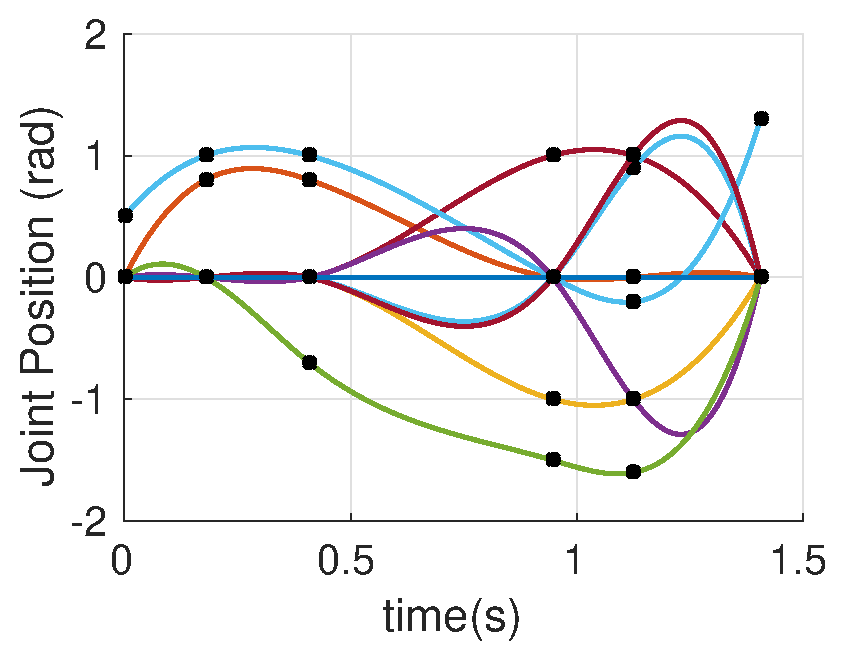
\includegraphics[width=0.7\textwidth]{keyframe}
\end{center}
\caption{Movimento keyframe utilizando interpolaçãpo por spline cúbica. Cada cor representa a trajetória de uma junta durante o movimento.}
\label{fig:keyframeData}
\end{figure}


\subsection*{Otimização de Movimentos Keyframe}

No caso particular de otimização de movimentos keyframe, o vetor  \( \mathrm{\mathbf{x}} \) é dado pelos parametros associados ao movimento keyframe \( \mathrm{\mathbf{m}} \). Além disso, precisa-se definir uma função de custo  \( f \left( \mathrm{\mathbf{x}} \right) \) que codifica a saída desejada do movimento keyframe (e.g. Chutar a bola o mais longe possível). dado que a saida do movimento keyframe depende de uma simulação, não é possível escrever uma expressão analítica para a função\( f\left( \mathrm{\mathbf{x}} \right) \). Portanto, resolver tal problema de otimização é particularmente complexo, exigindo uma boa avaliação da simulação do movimento. 

\begin{figure}[htb]

\begin{center}
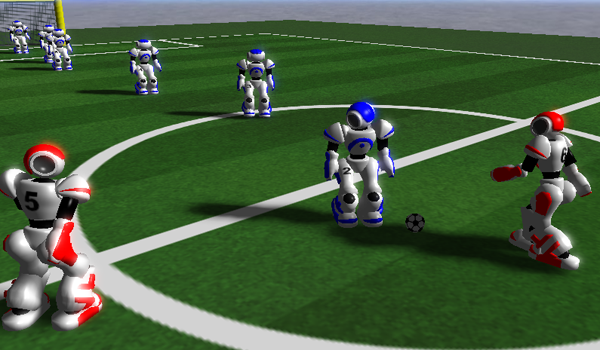
\includegraphics[scale=0.6]{game-screenshot.png}
\end{center}
\caption{\label{fig:simspark}RoboCup 3D Soccer Simulation com imagens retiradas no Monitor Roboviz.}
\end{figure}

\subsection{Framework de Otimização}
		
O framework contém os seguintes algoritmos de otimização implementados em MATLAB: Hill Climbing (HC), Particle Swarm Optimization (PSO), e Covariance Matrix Adaptation Evolution Strategy (CMA-ES). O algortimo HC foi implementado como visto em \cite{Russell:2003:AIM:773294} e o PSO tal como em \cite{Poli2007}. A implementação do CMA-ES é baseada na dada em \cite{cmaimpl}. Uma descrição do algoritmo de CMA-ES pode ser encontrada em \cite{cmatutorial}.

Pode-se notar que na otimização de movimentos keyframe, cada avaliação da função de custo requer uma simulação, portanto tal avaliação é o gargalo em tempo da otimização, e implementar tais algoritmos em uma linguagem mais rápida, tal como C++, não iria reduzir significativamente o tempo de otimização. 

O servidor de otimização acelera a otimização por paralelização. A arquitetura do servidor é apresentada na Fig. \ref{fig:serverDiagram}.

\begin{figure}[htb]
\begin{center}
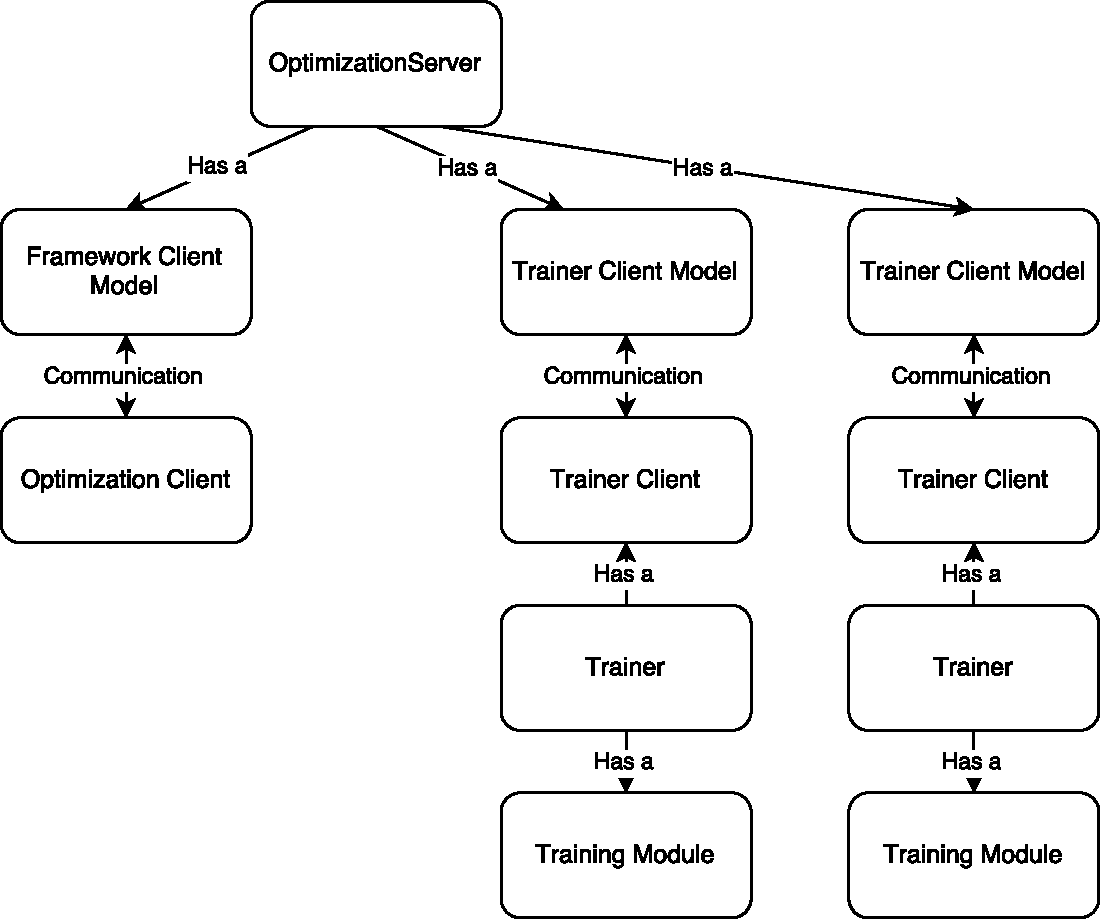
\includegraphics[scale=0.6]{diagramaServidorOtimizacao.pdf}
\end{center}
\caption{\label{fig:serverDiagram}Diagrama do framework de otimização.}
\end{figure}

O \inlinecode{OptimizationServer} recebe uma matriz  $\mathrm{\mathbf{X}} \in \mathbb{R}^{k\times p} $
do \inlinecode{OptimizationClient}, onde o algoritmo de otimização está rodando, e quebra tal matriz em \( p \) vetores $\mathrm{\mathbf{x}}_i \in \mathbb{R}^k, \ i = 1,\dots, p$, de tal maneira que cada vetor \( \mathrm{\mathbf{x}}_i \) representa um ponto no espaço de otimização (ou também pode ser chamado de partícula) que contem informação suficiente para avaliar o custo da função \( f \left( \mathrm{\mathbf{x}}_i \right) \).

O servidor funciona em um ambiente utilizando multiplas threads, onde cada vetor \( \mathrm{\mathbf{x}}_i \) a ser avaliado é enviado para uma thread \( T_i \).
Cada Thread do servidor comunica-se com um \inlinecode{Trainer} usando comunicação por socket de Linux. Um \inlinecode{Trainer} recebe um vetor \( \mathrm{\mathbf{x}}_i \) e usa um \inlinecode{TrainingModule} para computar o conjunto de saidas \( \mathrm{\mathbf{o}}_i \), que serão utilizadas pelo \inlinecode{OptimizationClient} para computar o valor de custo. O \inlinecode{TrainingModule} funciona como uma Caixa-preta para o respectivo \inlinecode{Trainer}. Portanto, um modulo de treinamento pode computar o conjunto de saídas de maneira arbitraria, incluindo situações em que é necessária uma simulação para calcular tais saídas.

As saídas são reunídas em uma matriz 
\( \mathrm{\mathbf{O}} = \left[ \mathrm{\mathbf{o}}_1, \mathrm{\mathbf{o}}_2, \dots, \mathrm{\mathbf{o}}_p \right] \) pelo servidor, e retornadas para o  \inlinecode{OptimizationClient}. Com isso, o  \inlinecode{OptimizationClient} usa a matriz \( \mathrm{\mathbf{O}} \) para computar o vetor de custos \( \mathrm{\mathbf{c}} = \left[ c_1, c_2, \dots, c_p \right] \in \mathbb{R}^p \), que e finalmente usado para atualizar os algoritmos de otimização e iniciar uma nova iteração dos algoritmos.

Dada tal arquitetura, para cada problema de otimização, será preciso apenas a criação de um novo modulo de treinamento, e um avaliador da função de custo. Isso pode ser facilmente realizado no framework, utilizando boas práticas de programação, tais como técnicas de Programação Orientada à Objetos.	

\subsection{Cluster}

Pode-se observar o cluster utilizado na Fig. \ref{fig:cluster}. O cluster utilizado é heterogêneo, tendo 4 computadores IPC2 i7, e 3 NUCs i5, sendo tais computadores, juntamente com o framework de otimização, utilizados para acelerar as otimizações.

\begin{figure}[htb]
\begin{center}
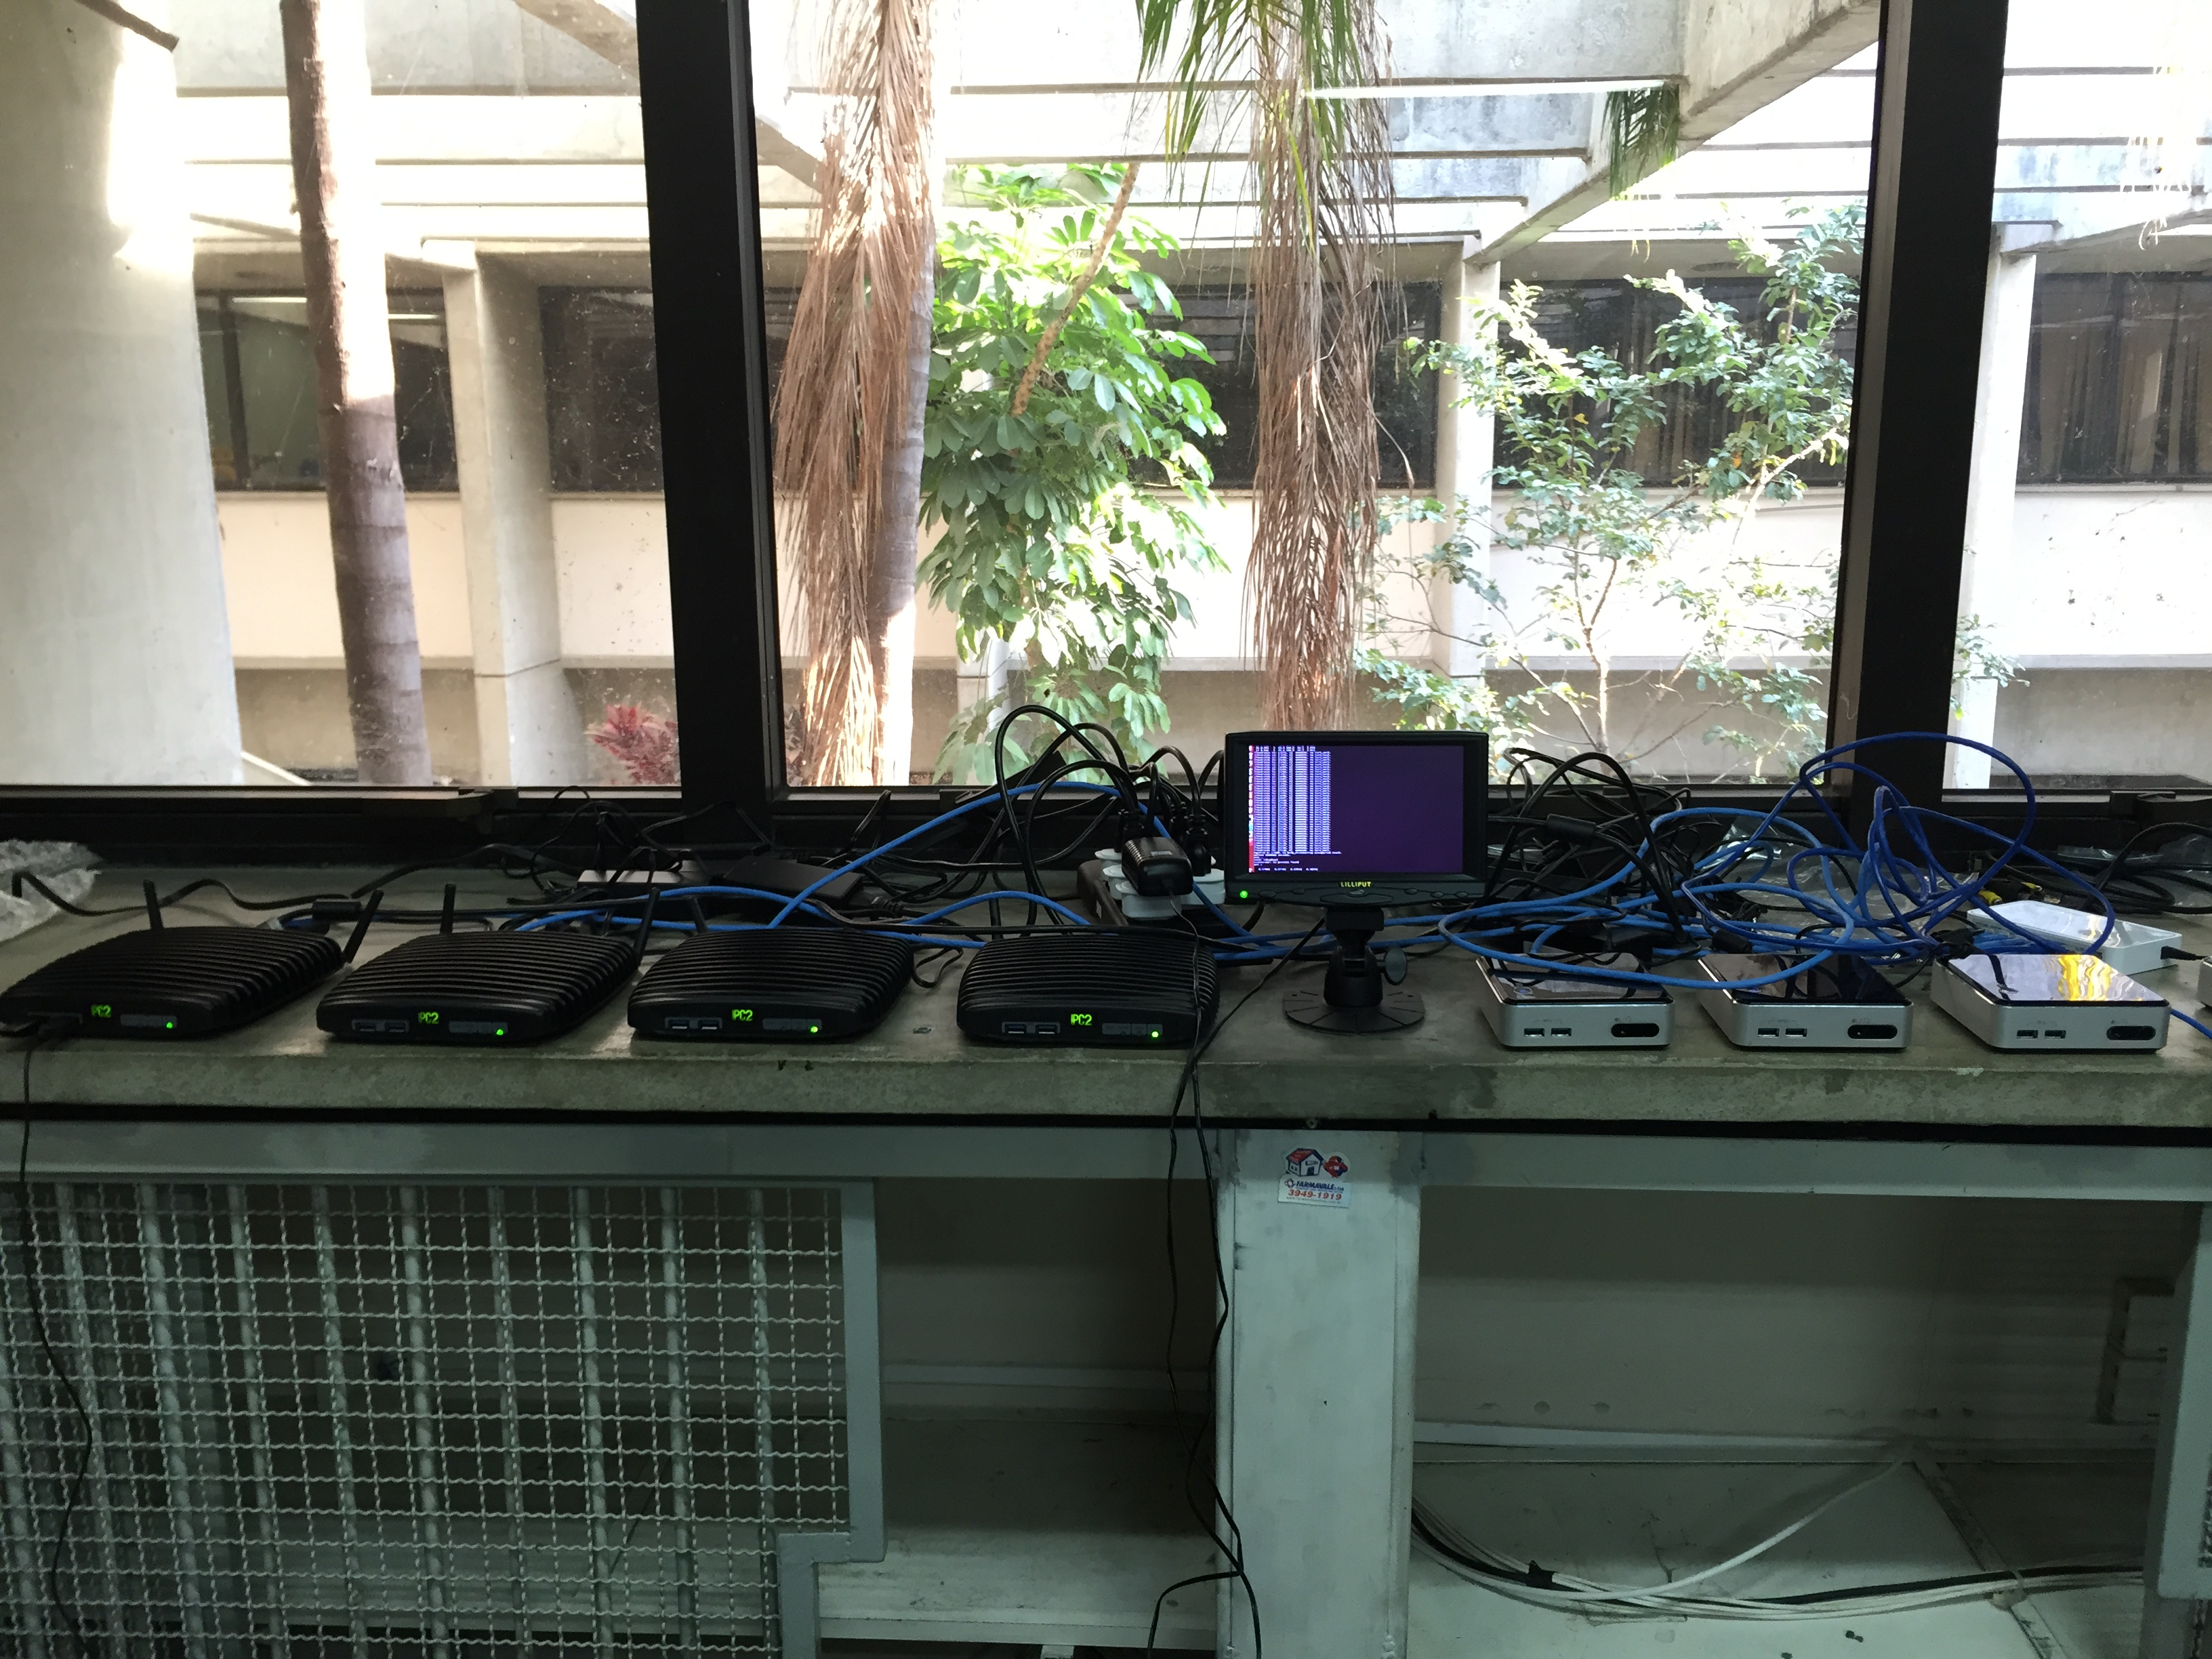
\includegraphics[width=1\textwidth]{image1.jpg}
\end{center}
\caption{\label{fig:cluster}Foto do cluster utilizado.}
\end{figure}

	
	


%----------------------------------------------------------------------------------------
%	RESULTADOS OBTIDOS
%----------------------------------------------------------------------------------------


\section{Resultados Obtidos}

\subsection{Otimizações feitas}
	
\subsubsection{Movimento de levantar de costas}

		O movimento $\mathrm{\mathbf{m}}_{standback} \in M$ foi inicialmente com $\gamma = 6$. O movimento inicial era suficiente para fazer o robô levantar, mas não tinha estabilidade.Portante, decidiu-se manter as posições de juntas e otimizar apenas os espaços de tempo. Com isso, os parametros selecionados para a otimização foram os valores $\mathrm{\mathbf{x}} = \left[ r, t_2, \dots, t_{7} \right]^T \in \mathbb{R}^7$, onde \( \mathrm{\mathbf{x}} \) é um ponto no espaço de otimização.

Sendo a simulação do Simpark intrinsicamente ruidosa, decidiu-se avaliar cada posição do espaço 10 vezes e tirar uma média dos valores de custo para diminuir o ruido. A função de custo é computada usando  \eqref{eq:standUpFromBack}.

\begin{equation} \label{eq:standUpFromBack}
f \left( \mathrm{\mathbf{x}} \right) = -w_{fall} b_{fall} + w_{time} \Delta t - w_{\overline{z}_{torso}} \overline{z}_{torso}
%	cost = -Penalty_{fall} - Time_{weight} t - MeanHeigth_{weight} * \overline{z}
\end{equation}
onde \( b_{fall} \) é um inteiro associado à informação do robô ter caido ou não, sendo -1 se o robô cair, e 1 se não cair, \( \Delta t \) é o tempo que o robô gasta para tentar levantar, e \( \overline{z}_{torso} \) é a altura média do torso do robô, sendo um parametro importante para descartar movimentos que ficam muito tempo parado no chão. Além disso, os pesos\( w_{fall} = 50 \), \( w_{time} = 10\), e \( w_{\overline{z}_{torso}} =1\) estão associados com o indicador de queda\( b_{fall} \), o tempo decorrido \( \Delta t \) e a altura média\( \overline{z}_{torso} \), respectivamente. Dada essa função de custo, o conjunto de saídas para esse problema de otimização é dado por\( \mathrm{\mathbf{o}} = \left[ b_{fall}, \Delta t, \overline{z}_{torso}  \right]^T \). Deseja-se deixar \( b_{fall} = 1 \), diminuir o tempo de levantar, e aumentar o valor de \( \overline{z}_{torso} \) para garantir que o robô ficou pouco tempo parado no chão.

O modulo de treinamento executou o procedimento descrito a seguir para computar a função de custo:
\begin{enumerate}
\item O robô é inicializado em uma posição fixa no campo.
\item Um movimento keyframe para fazer o robô cair com as costas para trás é executado.
\item O \inlinecode{StandUpFromBack} movement é executado para fazer o robô tentar levantar.
\item As saídas necessárias para calcular a função de custo são computadas.
\end{enumerate}

A Fig. \ref{fig:getUpBackOptimizationData} mostra a evolução dos valores melhores e medianos do conjunto de particulas avaliadas a cada iteração da otimização do movimento \inlinecode{StandUpFromBack}. O valor inicial encontrado é bom, entretanto o algoritmo CMA-ES evita uma convergência prematura para encontrar uma solução melhor, explorando melhor o espaço, e, percebe-se que o algoritmo consegue achar uma solução mais estável. A tabela \ref{tab:getUpBackTable} mostra dados comparando o movimento inicial e o otimizado, onde cada movimento é executado 1000 vezes. Nota-se que o movimento é mais estável que o inicial.

Em uma segunda otimização, conseguiu-se atingir um movimento um pouco mais estável, como pode ser visto na Fig. \ref{fig:getUpBackOptimizationData2}, usando a função de custo \eqref{eq:standUpFromBack2}, onde $w_{fall} = 20$ e $w_{time} = 10$.

\begin{equation} \label{eq:standUpFromBack2}
f \left( \mathrm{\mathbf{x}} \right) = -w_{fall} b_{fall} + w_{time} \Delta t
\end{equation}

 O movimento otimizado é descrito na Fig. \ref{fig:getUpBackFrames}.

\begin{table}
\centering
\caption{Comparação entre os movimentos otimizado e não otimizado.}
\label{tab:getUpBackTable}
\begin{tabular}{|l|l|l|}
\hline
Movimento      & Fração de sucesso & tempo(s)  \\ \hline
Não Otimizado & 0.80100  & 1.7  \\ \hline
Otimizado    & 0.93400  & 1.7  \\ \hline
\end{tabular}
\end{table}

\begin{figure}[htb]
\begin{center}
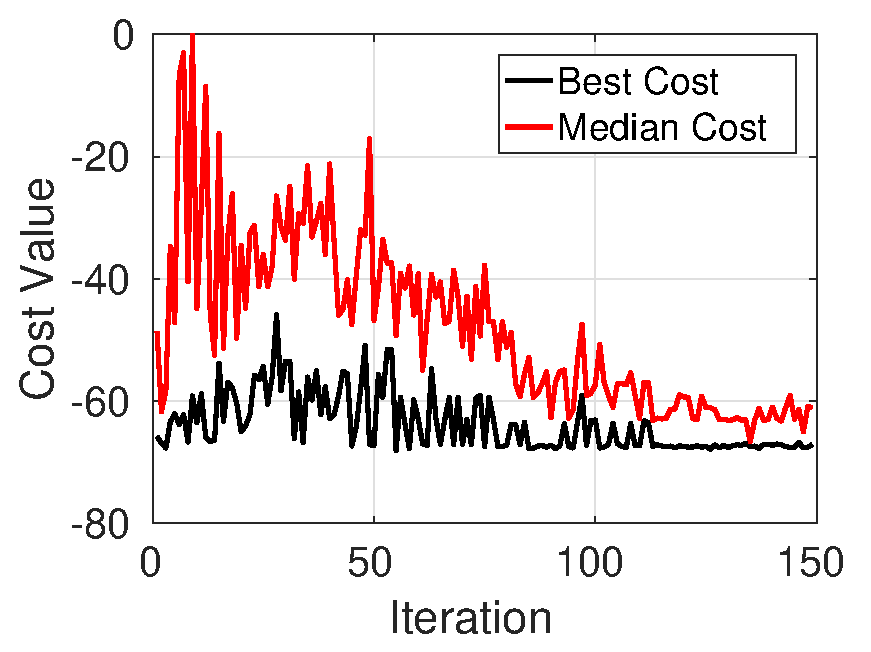
\includegraphics[scale=0.6]{getUpBackOptimization}
\end{center}
\caption{\label{fig:getUpBackOptimizationData}Evolução dos valores melhores e medianos de cada iteração do algoritmo de otimização para o movimento \inlinecode{StandUpFromBack}.}
\end{figure}

\begin{figure}[htb]
\begin{center}
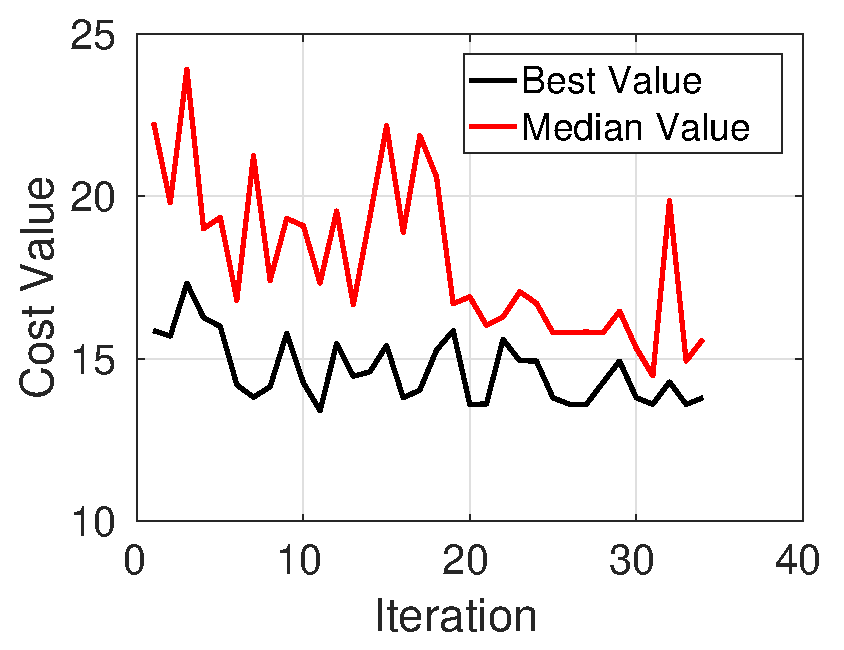
\includegraphics[scale=0.6]{otimizacaocostas2}
\end{center}
\caption{\label{fig:getUpBackOptimizationData2}Segunda Evolução dos valores melhores e medianos de cada iteração do algoritmo de otimização para o movimento \inlinecode{StandUpFromBack}.}
\end{figure}



\begin{figure*}
	\begin{center}
	      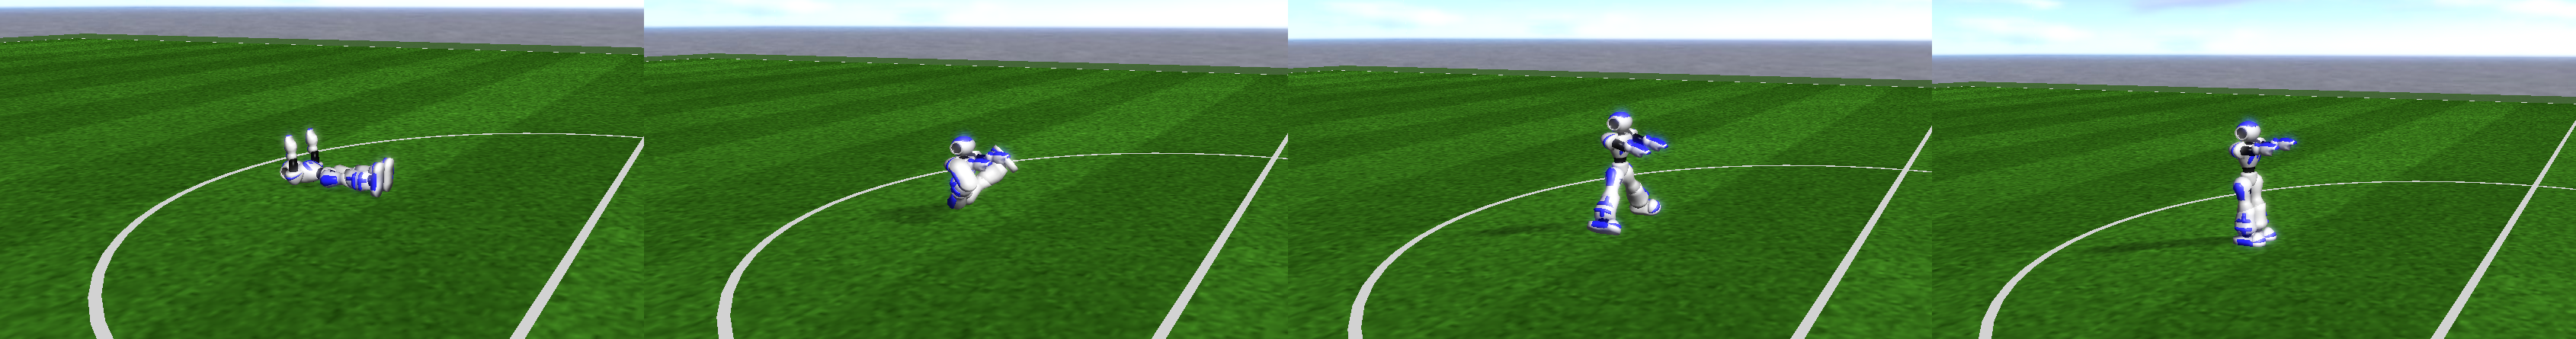
\includegraphics[width=1.0\textwidth]{getUpOptimizedFrame.png}
  \caption{Representação do movimento  \inlinecode{StandUpFromBack} em quadros.}
  \label{fig:getUpBackFrames}	
	\end{center}

\end{figure*}


	
	\subsubsection{Chute}
	
	O movimento \inlinecode{KickRightLeg}, para chutar a bola com a perna esquerda, $\mathrm{\mathbf{m}}_{kick} \in M$ tem $\gamma = 10$. A otimização foi feita considerando os passos de tempo e a taxa de velocidade como variáveis, portanto uma posição no espaço de otimização é dada por  $\mathrm{\mathbf{x}}_i = \left[ r, t_{2}, \dots, t_{\gamma =10} \right]^T$. As juntas não são consideradas na otimização por que a dimensionalidade do espaço de otimização seria muito grande. De maneira simila à otimização do movimento \inlinecode{StandUpFromBack}, cada posição foi avaliada 10 vezes utilizando a função de custo dada em \eqref{eq:kickRightLeg}.
\begin{equation} \label{eq:kickRightLeg}
 f \left( \mathbf{x} \right) = -w_{fall} * b_{fall} - w_x x + w_y \abs{y} - w_{\overline{z}_{ball}} \overline{z}_{ball}  
\end{equation}
Onde \( \overline{z}_{ball} \) é a altura média da bola, e é considerada pois se deseja um chute alto para não atingir adversários, e \( x \) e \( y \) são as coordenadas finais da posição da bola, respectivamente. O sistema de coordenadas é o mesmo utilizado pelo simulador do Simspakr, que é apresentado na Fig. \ref{fig:referenciaCamp}. Além disso, os pesos \( w_x = 10 \), \( w_y = 10 \), e \( w_{\overline{z}_{ball}} = 5\) estão associados aos dados de \( x \), \( y \), e \( \overline{z}_{ball} \), respectivamente. Nesse caso, o modulo de treinamento rodou a seguinte simulação 10 vezes para cada partícula:
%
\begin{enumerate}

	\item 	O robô foi inicializado na posição \( \left( -0.2,0.1 \right) \).
	\item A bola foi colocada na posição \( \left( 0,0 \right) \).
	\item Então o robô tentou executar o movimento \inlinecode{KickRightLeg}.
\item Os dados necessários para calcular o custo da função são armazenados.
\end{enumerate}

\begin{figure}[htb]
\begin{center}
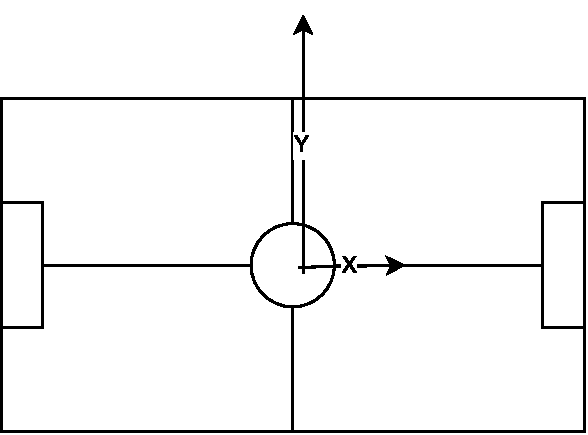
\includegraphics[width=0.48\textwidth]{FieldDiagram.pdf}
\end{center}
\caption{\label{fig:referenciaCamp}Diagrama de referência para o campo.}
\end{figure}

A Fig. \ref{fig:kickRightLegOptimizationData} mostra a evolução dos valores melhores e medianos do conjunto de posições avaliadas a cada iteração da otimização para o movimento \inlinecode{KickRightLeg}. 

Além desse chute inicial adquirido, conseguiu-se outro chute, que apresentava melhores resultados, e otimizou-se sobre tal chute, tendo os valores apresentados na Fig. \ref{fig:kickRightLegOptimizationData2}, com a função de custo dada em \eqref{eq:kickRightLeg2}, onde 
 $ x_{g} = 10, y_{g} = 0, w_{exp} = 100$ , $w_{x} = 10$ e $w_{y}=5$ são a posição objetivo em x, em y, o peso  associado à exponencial, à diferença em x e a diferença em y.

\begin{equation} \label{eq:kickRightLeg2}
 f \left( \mathbf{x} \right) = -w_{exp}  e^{-\abs{(w_{x}(x-x_{g}),w_{y}(y-y_{g}))}}
\end{equation}
		
\begin{figure}[htb]
\begin{center}
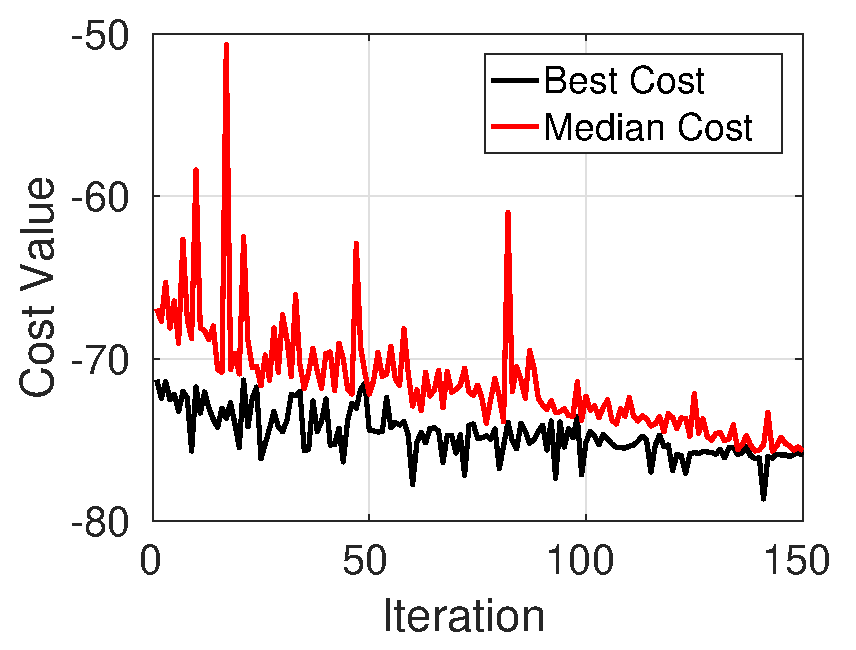
\includegraphics[width=0.6\textwidth]{kickRightLegOptimization}
\end{center}
\caption{\label{fig:kickRightLegOptimizationData}Evolução dos valores melhores e medianos de cada iteração do algoritmo de otimização para o movimento \inlinecode{KickRightLeg}.}
\end{figure}

\begin{figure}[htb]
\begin{center}
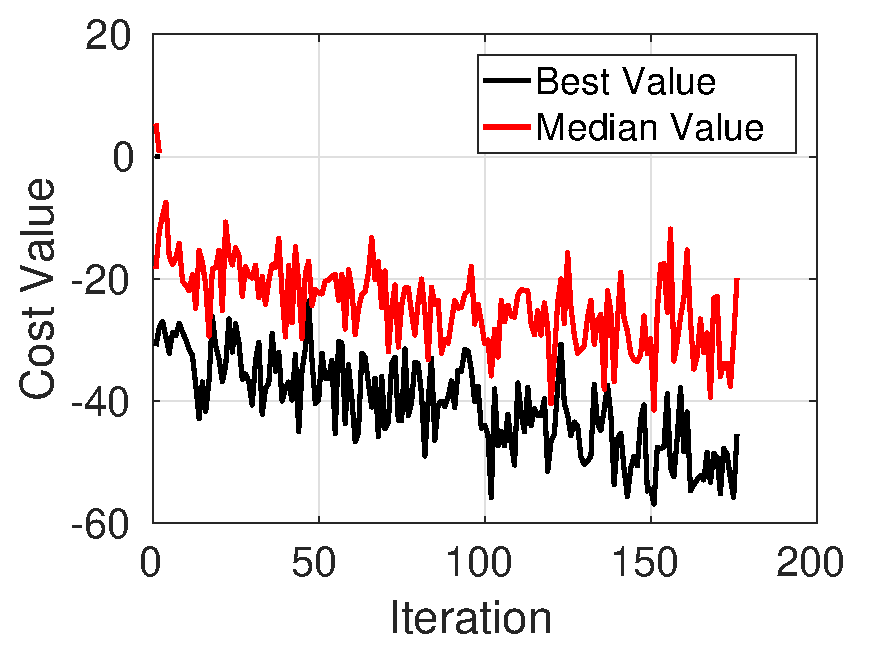
\includegraphics[width=0.6\textwidth]{otimizacaokick2}
\end{center}
\caption{\label{fig:kickRightLegOptimizationData2}Segunda evolução  dos valores melhores e medianos de cada iteração do algoritmo de otimização para o movimento \inlinecode{KickRightLeg} .}
\end{figure}
	   
	    		
		
%----------------------------------------------------------------------------------------
%	CONCLUSÕES
%----------------------------------------------------------------------------------------
	

\section{Conclusões}

	Percebe-se que, com o framework desenvolvido, conseguiu-se diminuir o tempo necessário para a otimização dos movimentos de robô humanoide, resolvendo de maneira simples e de fácil implementação. 
	
	Além disso, pode-se ver a melhoria do Time da ITAndroids, com tais otimizações feitas, ajudando o time de Soccer3D a ficar mais competitivo.

%----------------------------------------------------------------------------------------
%	AGRADECIMENTOS
%----------------------------------------------------------------------------------------

\section{Agradecimentos}

Gostaria-se de agradecer ao CNPQ, pela oportunidade oferecida e o auxílio dado
à pesquisa realizada. Agradece-se também ao professor Carlos Henrique Costa Ribeiro,
professor orientador da inicação cientifica, por todo o apoio dado à pesquisa, e ajuda no
desenvolvimento do projeto.

Agradecimentos a equipe de robótica ITAndroids, especialmente o time de Soccer3D juntamente com o Professor
Marcos Ricardo Omena de Albuquerque Maximo, que ajudaram no desenvolvimento das
ferramentas necessárias para a pesquisa.
Agradecimentos ao professor Paulo André Lima de Castro por oferecer o uso do
Frank Cluster, um cluster de computadores da Divisão de Computação do ITA, que ajudou no início do projeto.

Agradecimentos a Divisão de Computação do ITA, e especialmente ao LAB-SCA, que forneceu o equipamento para o cluster para as otimizações finais e ao técnico Carlos que ajudou na montagem do cluster.


%------------------------------------------------



%----------------------------------------------------------------------------------------
%	BIBLIOGRAPHY
%----------------------------------------------------------------------------------------


\bibliographystyle{unsrt}

\bibliography{sample.bib} % The file containing the bibliography

%----------------------------------------------------------------------------------------

\end{document}